\chapter{Electrodynamique}

\section{Un exercice pédagogique}
\subsection{Générateur et circuit électrique}
%\subsection{Effet joule}
\begin{minipage}[c]{.5\linewidth}
\hspace{0.7cm}Un générateur électrique G (pile électrochimique) maintient une tension électrique (ou force électromotrice) U entre ses bornes. Cette tension produit un courant électrique I dans le circuit électrique contenant des fils de résistance négligeable et le conducteur ohmique R.
\end{minipage}
\hfill
\begin{minipage}[c]{.5\linewidth}
\begin{center}
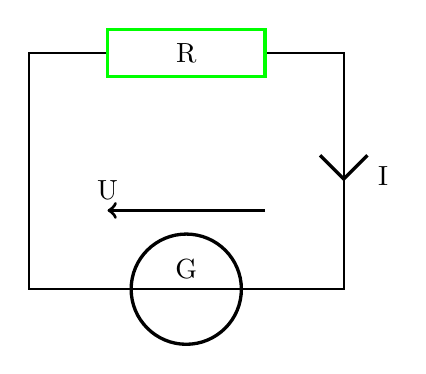
\begin{tikzpicture}
\draw [very thick] (0,0) node [above]{G} circle(0.7);
\draw [->, very thick] (1,1) -- (-1,1) node [above]{U};
\draw [thick] (-1,3) -- (-2,3) -- (-2,0) -- (2,0) -- (2,3) -- (1,3);
\draw [very thick, green] (-1,3.3) -- (-1,2.7) -- (1,2.7) -- (1,3.3) -- cycle;
\draw (0,3) node {R};
\draw [very thick] (2.3,1.7) node [below right]{I} -- (2,1.4) -- (1.7,1.7);
\end{tikzpicture}
\end{center}
\end{minipage}\vspace{0.5cm}

L'expérience montre que la température du conducteur ohmique s'élève, c'est l'effet Joule. Nous nous interressons aux transferts d'énergie responsable de cet échauffement :

Dans le générateur, de l'énergie électrochimique est convertie en énergie électrique, dans le conducteur ohmique de l'énergie électrique est convertie en énergie thermique. Nous souhaitons interpréter et évaluer cette dernière conversion.

Le conducteur ohmique R est cylindrique (longueur {\it l}, section {\it s}). La tension U est maintenue entre ses extrémités, il est parcouru par le courant I (le courant I est proportionnel à la tension U. C'est la loi d'Ohm : U $=$ R.I).

\begin{center}
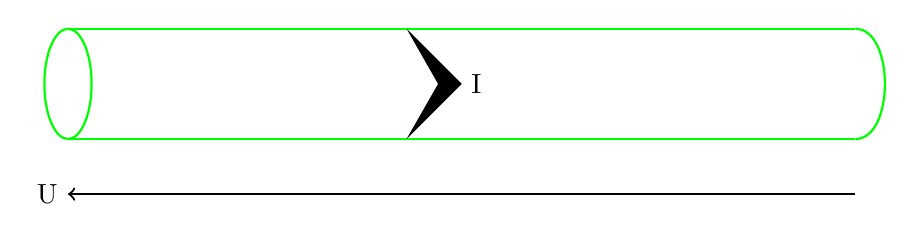
\begin{tikzpicture}
\draw[thick, green] (0,0) ellipse (0.3cm and 0.7cm);
\draw[thick, green] (0,0.7) -- (10,0.7);
\draw[thick, green] (0,-0.7) -- (10,-0.7);
\draw [thick,->] (10,-1.4) -- (0,-1.4) node [left] {U};
\fill (5,0) -- (4.3,0.7) -- (4.7,0) -- (4.3,-0.7) -- cycle node [right] {I};
\draw[thick, green] (10,0.7) .. controls (10.5,0.7) and (10.5,-0.7) .. (10,-0.7);
\end{tikzpicture}
\end{center}

La tension U est une différence de potentiel entre les extrémité du conducteur ohmique, relié par définition au champ électrique {\bf E}

\subsection{Électrons libres et champ électrique}
Au niveau microscopique, le conducteur ohmique est constitué par un réseau d'ions positifs fixes

\begin{tikzpicture}
\draw (0,0) node [color=red] {$+$};\draw (0,0) [thick, color=gray!40] circle (0.3);
\end{tikzpicture}
et d'électrons mobile
\begin{tikzpicture}
\draw (0,0) node [color=blue] {$e^-$};
\end{tikzpicture}. L'ensemble étant électriquement neutre.
\begin{center}
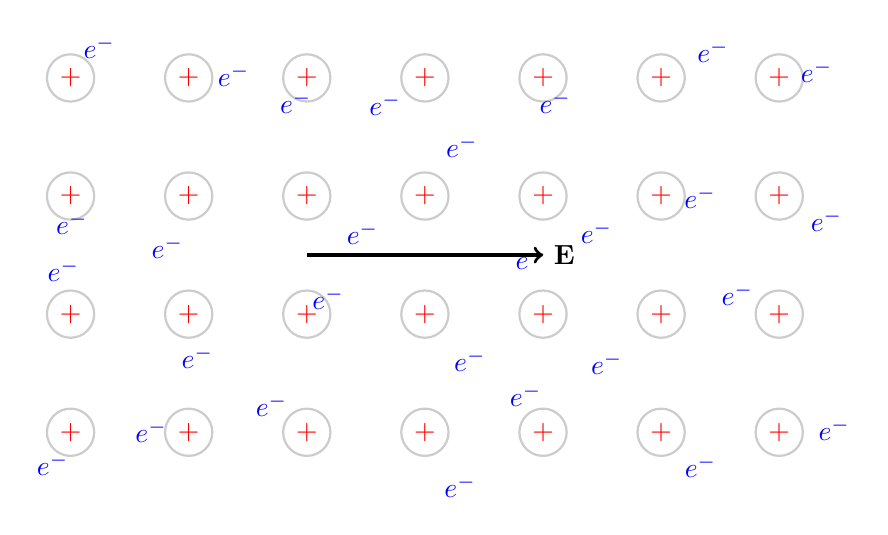
\begin{tikzpicture}
\foreach \x in {-2,-0.5,...,3}
{\foreach \y in {1,2.5,...,11}
{\draw (\y,\x) node [color=red] {$+$};\draw (\y,\x) [thick, color=gray!40] circle (0.3);
%\draw (\y+0.75+0.3*rand,\x+0.75+0.3*rand) node {$e^-$};}}
\draw (\y+0.75*rand,\x+0.75*rand) node [color=blue] {$e^-$};}}
\draw [->, very thick] (4,0.25) -- (7,0.25) node [right] {{\bf E}};
\end{tikzpicture}
\end{center}
Le courant électrique est due au mouvement d'ensemble des électrons mobiles (libres) sous l'effet du champ électrique {\bf E} ( relié par définition à la tension U
% : {\bf E} $=-\frac{\partial}{\partial\mt{x}}$V(x)$\hat{\mt{x}}$
).

Soumis à une force de la part du champ électrique, les électrons libres sont mis en mouvement. Ils subissent alors des collisions avec les ions immobile, leurs cédant une partie de leur énergie cinétique. Les ions du réseau acquièrent alors de l'énergie de vibration, se traduisant par un échauffement du conducteur.

\subsection{Champ magnétique et vecteur de Poynting}

Le courant I produit un champ magnétique : Les lignes de champs sont des cercles, centré sur l'axe du conducteur, le champ est perpendiculaire à cet axe.

\vspace{0.5cm}
\begin{minipage}[c]{.45\linewidth}
\begin{center}
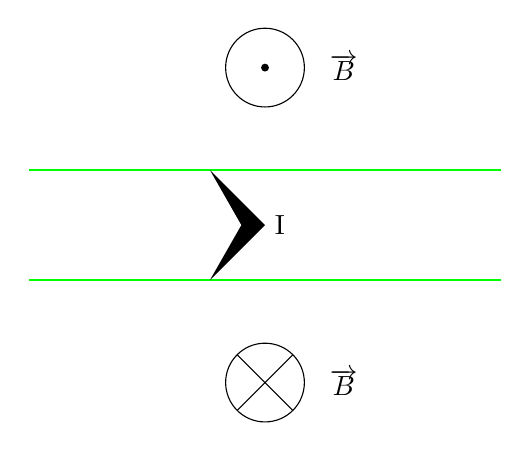
\begin{tikzpicture}
\draw [thick, green] (2,0.7) -- (8,0.7);
\draw [thick, green] (8,-0.7) -- (2,-0.7);
\fill (5,0) -- (4.3,0.7) -- (4.7,0) -- (4.3,-0.7) -- cycle node [right] {I};
\draw (5,2) circle(0.5);
\fill (5,2) circle(0.05);
\draw (6,2) node {$\overrightarrow{\mt{B}}$};
\draw (5,-2) circle(0.5);
\draw (5.35,-2.35) -- (4.65,-1.65);
\draw (5.35,-1.65) -- (4.65,-2.35);
\draw (6,-2) node {$\overrightarrow{\mt{B}}$};
\end{tikzpicture}

Vue dans un plan parallèle à l'axe du conducteur
\end{center}
\end{minipage}
\hfill
\tikzstyle{fleche}=[->,line width=3pt]
\begin{minipage}[c]{.45\linewidth}
\begin{center}
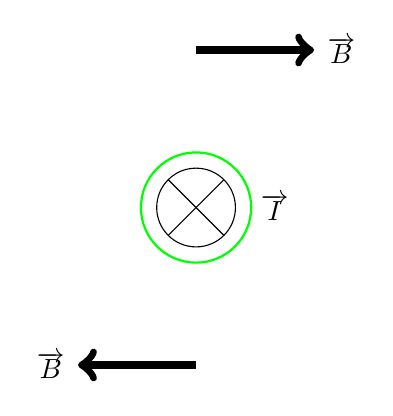
\begin{tikzpicture}
\draw[thick, green] (0,0) circle(0.7);
\draw (0,0) circle(0.5);
\draw (0.35,0.35) -- (-0.35,-0.35);
\draw (-0.35,0.35) -- (0.35,-0.35);
\draw (1,0) node {$\overrightarrow{\mt{I}}$};
\draw [fleche] (0,2) -- (1.5,2) node [right] {$\overrightarrow{\mt{B}}$};
\draw [fleche] (0,-2) -- (-1.5,-2) node [left] {$\overrightarrow{\mt{B}}$};
\end{tikzpicture}

Vue dans un plan perpendiculaire à l'axe du conducteur
\end{center}
\end{minipage}

\vspace{0.5cm}
\begin{minipage}[c]{.45\linewidth}
\begin{center}
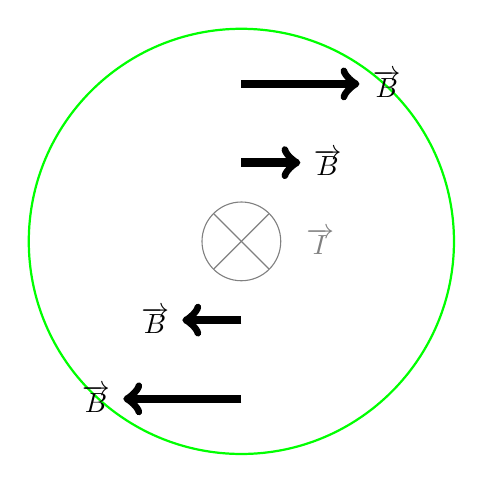
\begin{tikzpicture}
\draw[thick, green] (0,0) circle(2.7);
\draw[thin, gray] (0,0) circle(0.5);
\draw[thin, gray] (0.35,0.35) -- (-0.35,-0.35);
\draw[thin, gray] (-0.35,0.35) -- (0.35,-0.35);
\draw (1,0) node[color=gray] {$\overrightarrow{\mt{I}}$};
\draw [fleche] (0,2) -- (1.5,2) node [right] {$\overrightarrow{\mt{B}}$};
\draw [fleche] (0,1) -- (0.75,1) node [right] {$\overrightarrow{\mt{B}}$};
\draw [fleche] (0,-2) -- (-1.5,-2) node [left] {$\overrightarrow{\mt{B}}$};
\draw [fleche] (0,-1) -- (-0.75,-1) node [left] {$\overrightarrow{\mt{B}}$};
\end{tikzpicture}
\end{center}
\end{minipage}
\hfill
\tikzstyle{fleche}=[->,line width=3pt]
\begin{minipage}[c]{.45\linewidth}
À l'intérieur du conducteur, le champ magnétique est nul sur l'axe, son amplitude augmente en s'écartant de l'axe :
\end{minipage}
\vspace{0.5cm}

\vspace{0.5cm}
\begin{minipage}[c]{.45\linewidth}
On constate que le champ magnétique est perpendiculaire au champ électrique. On en déduit le sens et la direction du vecteur de Poyting :
\end{minipage}
\hfill
\tikzstyle{fleche}=[->,line width=3pt]
\begin{minipage}[c]{.45\linewidth}
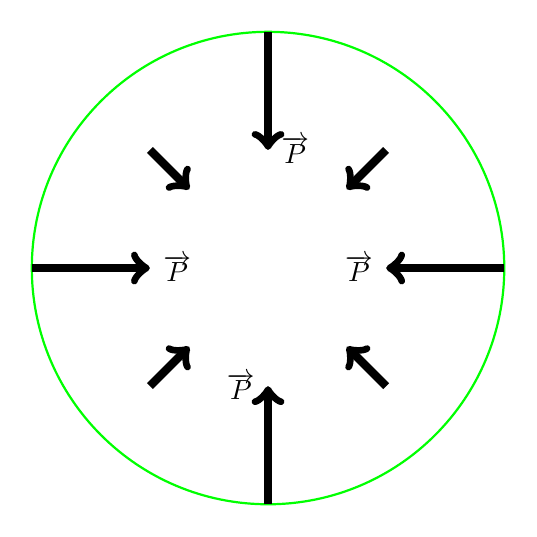
\begin{tikzpicture}
\draw[thick, green] (0,0) circle(3);
\draw [fleche] (0,3) -- (0,1.5) node [right] {$\overrightarrow{\mt{P}}$};
\draw [fleche] (3,0) -- (1.5,0) node [left] {$\overrightarrow{\mt{P}}$};
\draw [fleche] (0,-3) -- (0,-1.5) node [left] {$\overrightarrow{\mt{P}}$};
\draw [fleche] (-3,0) -- (-1.5,0) node [right] {$\overrightarrow{\mt{P}}$};
\draw [fleche] (-1.5,-1.5) -- (-1,-1);
\draw [fleche] (1.5,1.5) -- (1,1);
\draw [fleche] (-1.5,1.5) -- (-1,1);
\draw [fleche] (1.5,-1.5) -- (1,-1);
%\draw [fleche] (1.5,1.5) -- (1.5,0) node [right] {$\overrightarrow{\mt{P}}$};
%\draw [fleche] (1.5,1.5) -- (0,-1.5) node [left] {$\overrightarrow{\mt{P}}$};
%\draw [fleche] (1.5,1.5) -- (-1.5,0) node [left] {$\overrightarrow{\mt{P}}$};
\end{tikzpicture}
\end{minipage}
\vspace{0.5cm}

L'amplitude du vecteur de Poyntig diminue lorsque l'on s'approche de l'axe. On en déduit que de l'énergie électromagnétique est cédée au conducteur. C'est de l'énergie électrique convertie en énergie thermique.

Cette conversion provoque l'échauffement du conducteur.
\subsection{Question}
La question qui se pose est : "qu'en est-il de l'effet Joule, à quoi est due l'échauffement du conducteur" : Faut-il considérer l'effet Joule comme la superposition des deux phénomènes
\begin{itemize}[leftmargin=1cm, label=\ding{32}, itemsep=1pt]
\item {\bf collision électron-ions :} les électrons mobile cèdent de l'énergie au réseau ionique,
\item {\bf vecteur de Poyting :} le champ électromagnétique cède de l'énergie au conducteur ?
\end{itemize}

